%%This is a very basic article template.
%%There is just one section and two subsections.
\documentclass{article}

\usepackage{cite}
\usepackage{graphicx}
\usepackage{caption}
\usepackage{subcaption}
\usepackage[a4paper, total={6in, 8in}]{geometry}

\begin{document}
\title{Self Consistent ill-posed Inverse Pronlem With Evolutionary Algorithm}
\maketitle

\section{Introduction}
In principle, ill-posed inverse problem with the regularization method can give
out a very good reconstructed result, but in practice, this is not always the
case. The main reason is that we apply our regularization method on the basis of
the given, noisy measured value.

In order to solve the ill-posed inverse problem
which the measure value or the model is not accurate enougth to give out a good reconstructed result, we
introduce the self consistent regularization method With Cross Validation.
\section{Methodology}
\subsection{Fredholm integral equation of the first kind}
A Fredholm integral equation of the first kind is an integral equation of the
form.
\begin{equation}
f(x) = \int\limits_a^b {K(x,t)\phi (t)dt}
\label{eq:firsttypeintegral}
\end{equation}
Where \(K(x,t)\) if the kerel and \(\phi (t)\) is an unknown function to be
solved for \cite{arfken2013mathematical}.

The first step to obtain a numerical solution of Eq.\ref{eq:firsttypeintegral}
is to change the integral equation to matrix form by applying discretization
method. There are two basically different approaches (Quadrature Methods and
Expansion Methods) to do this \cite{hackbusch2012integral}. In this work, we use
quadrature methos for simplicity and easy to implement.

After the discretization, Eq.\ref{eq:firsttypeintegral} becomes a linear system.
\begin{equation}
Ax = b
\label{eq:discreteintegral}
\end{equation}
The elements of the matrix A, the right-hand sized b, and the solution vector x
are given by
\begin{equation}
\left. {\begin{array}{*{20}{c}}
{{a_{ij}} = {\omega _j}K({x_i},{t_j})}\\
{{x_j} = \tilde \phi ({t_j})}\\
{{b_i} = f({x_i})}
\end{array}} \right\}\begin{array}{*{20}{c}}
{}&{i,j = 1,...,n.}
\end{array}
\end{equation}
It is known that linear system arising from the first kind Fredholm integral
equation such as Eq.\ref{eq:firsttypeintegral} are likely to be ill-conditioned
\cite{neumaier1998solving}.
\subsection{Singular Value Decomposition (SVD) analysis and Picard condition}
The singluar value decomposition (SVD) is a very powerful tool for analyzing
first kind Fredholm integral equation in the
discrete setting as shown in
Eq.\ref{eq:discreteintegral}\cite{trefethen1997numerical}.

In this work, we treat the matrix A as a square matrix \(A \in {R^{N \times
N}}\), and therefore the SVD of A takes the form
\begin{equation}
A = U\sum {V^T} = \sum\limits_{i = 1}^N {{u_i}{\sigma _i}v_i^T} 
\end{equation}
where \(\sum  \in {R^{N \times N}}\) is a diagonal matrix with the singular
values, satisfying
\[\sum  = diag({\sigma _1},...,{\sigma _n}),\begin{array}{*{20}{c}}
{}&{{\sigma _1} \ge {\sigma _2} \ge  \cdots  \ge {\sigma _n} \ge 0}
\end{array}\]
The matrix \(U \in {R^{n \times n}}\) and \(V \in {R^{n \times n}}\) consist of
the left and right singular vectors
\[U = ({u_1},...,{u_N}),\begin{array}{*{20}{c}}
{}&{V = ({v_1},...,{v_N})}
\end{array}\]
After we have performed SVD on the matrix A, the solution of x in
Eq.\ref{eq:discreteintegral} takes the form
\begin{equation}
x = {A^{ - 1}}b = \sum\limits_{i = 1}^N {\frac{{u_i^Tb}}{{{\sigma _i}}}{v_i}}
\end{equation}
For a stable solution x to exist, the right-hand side coefficients \(u_i^Tb\)
must decay to zero faster than the singular values \({\sigma _i}\), a situation
that is referred to as the Picard condition. The violation of the Picard
condition is the simple explanation of the instablility of the inverse problem,
but it also gives a way to deal with it, by employing the regularization method.
\subsection{Regularization Method}
\subsubsection{Truncated Singular Value Decomposition}
From the discussion in the previous section, we compute a regularized
approximate solution by simply eliminating those SVD componets where the
\(u_i^Tb\) decay to zero more slowly than the sinular values \({\sigma _i}\).
Hence we define the truncated SVD (TSVD) solution obtained by:
\begin{equation}
{x_k} = \sum\limits_{i = 1}^k {\frac{{u_i^Tb}}{{{\sigma _i}}}{v_i}}
\end{equation}
The truncation parameter k should be choosen such taht all the noise-dominated
SVD coefficients are discarded. The value of k can be found from an inspection
of the Picard plot.
\subsubsection{Tikhonov Regularization}
TSVD method is very intutitive. The disadvantage is thart it explicityly
requires the computation of the SVD. This computation task can be too
overwhelming for large-scale problems. Therefore, we need another regularization
method which is suited for large computational problem which is the Tikhonov
Regularization mehtod.

The Tikhonov solution \({x_\lambda }\) is defined as the solution to the problem
\begin{equation}
\mathop {\min }\limits_x \left\{ {\left\| {Ax - b} \right\|_2^2 + {\lambda
^2}\left\| x \right\|_2^2} \right\}
\label{eq:tikhonovreqularization}
\end{equation}

where, the first term \(\left\| {Ax - b} \right\|_2^2\) measures the
goodness-of-fit, and the second term \(\left\| x \right\|_2^2\) measures the
regularity of the solution. The balance between the two terms is controlled by
the factor \({\lambda ^2}\).

The solution of Eq.\ref{eq:tikhonovreqularization} cam also be rewritten as
follows in terms of the SVD \cite{hansen2010discrete}.

\begin{equation}
{x_\lambda } = \sum\limits_{i = 1}^n {\varphi _i^{[\lambda
]}\frac{{u_i^Tb}}{{{\sigma _i}}}{v_i}}
\end{equation}
where \(\varphi _i^{[\lambda ]}\) is the filter factors and takes the form
\[\varphi _i^{[\lambda ]} = \frac{{\sigma _i^2}}{{\sigma _i^2 + {\lambda ^2}}} \approx \left\{ {\begin{array}{*{20}{c}}
1&{{\sigma _i} \gg \lambda }\\
{\sigma _i^2/{\lambda ^2}}&{{\sigma _i} \ll \lambda }
\end{array}} \right.\]

\subsection{Noise Analysis}
Assuming all the error comes from the Eq.\ref{eq:discreteintegral} is from the
right hand side b
\[b = {b^{exact}} + e\]
assuming e is a white noise.

In order to solve the Eq.\ref{eq:tikhonovreqularization} with the noise biased
right hand side b, we need to choose the factor \(\lambda \). The Discrepancy
Principle \cite{hoekstra2010simulating} shows that we should choose the factor
\(\lambda \) such that the residual norm \({\left\| {A{x_\lambda } - b}
\right\|_2}\) equals the ``discrepancy'' in the data, as measured by
\({v_{dp}}{\left\| e \right\|_2}\), where \({v_{dp}}\) is the ``safety factor''.
\begin{equation}
{\left\| {A{x_\lambda } - b} \right\|_2} = {v_{dp}}{\left\| e \right\|_2}
\label{eq:discrepancy}
\end{equation}

From Eq.\ref{eq:discrepancy}, we know that the goodness-of-fit of the problem is
dependent on the error from the right hand side b. The larger the error, the
worse the fit. This is the main challenge of using regularized method to solve
the inverse problem. If the error from the right hand side is too large, we can
only choose a relative large \(\lambda \) to discard the noise-dominated part,
which also discard large amound of useful information to reconstruct x.

In order to solve the problem when the noise from the right hand side b cannot
be ignored, we introduced a self consistent denoise technique to pre filter the
noise. We will search the space \(b \pm \eta \), where \(\eta \) is the standard
deviation of the white noise as shown in Fig.\ref{fig:bsearchspace}, and find
the combination can give us the least residual \({\left\| {A{x_\lambda } - b} \right\|_2}\) to form the new b which
is very close to \({b^{exact}}\).
Then we can feed the new b into the regularization process, which can give us a better reconstruct result.
 \begin{figure}[h!]
  \centering
    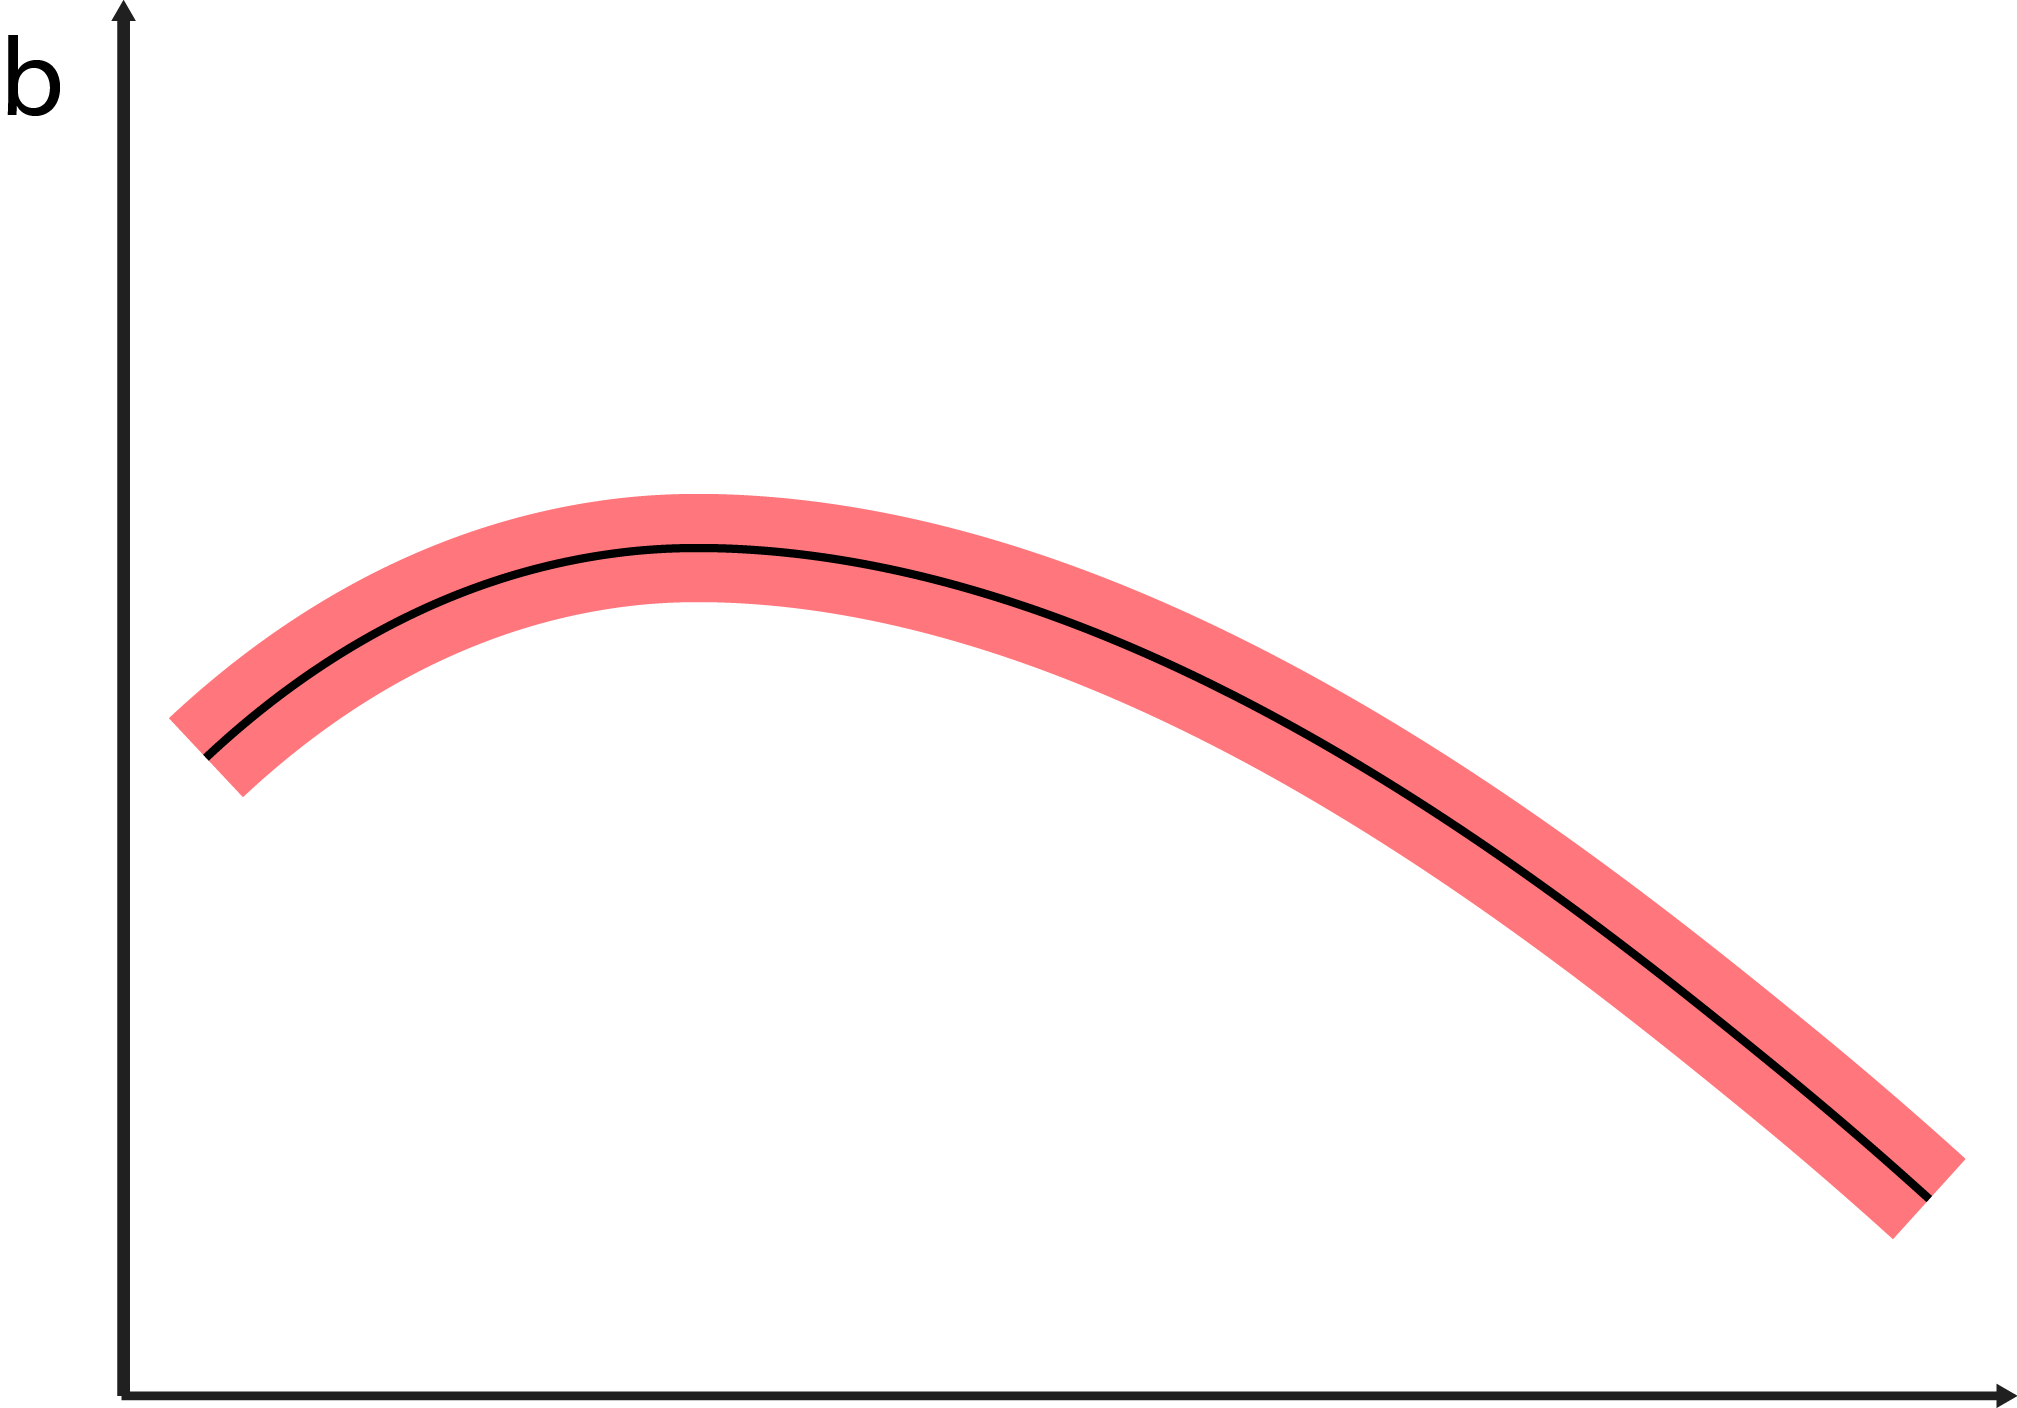
\includegraphics[width=0.7\textwidth]{images/bsearchspace/bsearchspace}
  \caption{The search space for \({b^{exact}}\), the black line is the measured
  b with noise, the red region is the search sapce, with a width \(2\eta \)}
  \label{fig:bsearchspace}
\end{figure}
Since the search space is a continuous space and can be very large, there is no
way to use brute force, or normal search algorithm to search the noise space.
We need to use a stochastic search algorithm. Evolutionary Algorithm is the most
famous stochastic search algorithm. In this work we use it to search the noise
space and find the least residual \({\left\| {A{x_\lambda } - b} \right\|_2}\).
\subsection{Evolutionary Algorithm}
\section{Numerical Results and Discussion}
We use a very simple model to illustrate how we use regularization method to
solve the ill-posed inverse problem. We use a simplified problem from gravity
surveying. An unknown mass distribution with density \(f(t)\) is located at
depth de below the surface. From 0 to 1 on the \(t\) axis shown in
Figure. \ref{fig:GeophysicsIllustrator}. We assume there is no mass outside
this source, which produce a gravity field everywhere. At the surface, along the
s axis in Figure. \ref{fig:GeophysicsIllustrator} from 0 to 1, we mreasure the
vertical component of the gravity field, which reger to as g(s).
 
 \begin{figure}[h!]
  \centering
    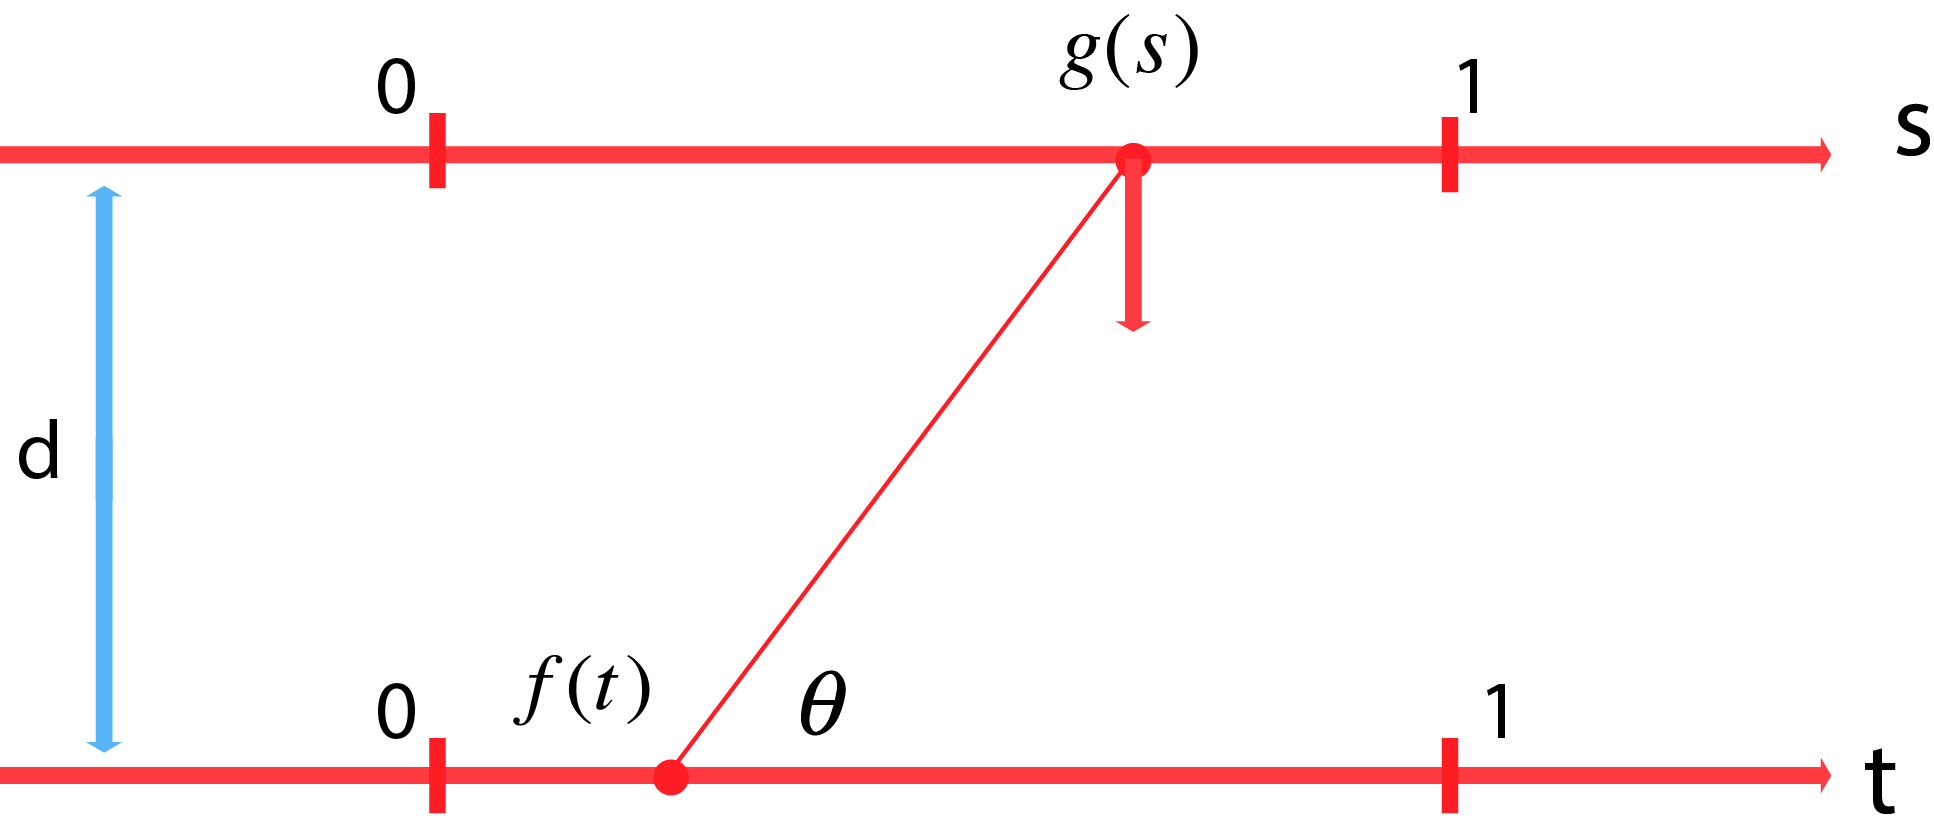
\includegraphics[width=0.7\textwidth]{images/GeophysicsIllustrator/illustrator}
  \caption{The geometry of the gravity surveying model problem: \(f(t)\) is the
  mass density at \(t\). and g(s) is the vertical component of the gravity
  field at s.}
  \label{fig:GeophysicsIllustrator}
\end{figure}
The two functions f and g are related via a Fredholm integral equation of the
first kind. The gravity field from an infinitesmally small part of f(t), of
length dt, on the axis is identical to the field from a point mass at t of
strength f(t)dt. Hence, the magnitude of the gravity field along s is
\(f(t)dt/{r^{2x}}\), where \(r = \sqrt {{d^2} + {{(s - t)}^2}} \) is the
distance between the source point at t and the field point at s. The direction
of the gravity field is from the field point to  he source point, and therefore
the measured value of g(s) is
\[dg = \frac{{\sin \theta }}{{{r^2}}}f(t)dt\]
where \(\theta \) is the angle shwon in Figure. \ref{fig:GeophysicsIllustrator}.
Using that \(\sin \theta  = d/r\), we obtain
\[\frac{{\sin \theta }}{{{r^2}}}f(t)dt = \frac{d}{{{{({d^2} + {{(s -
t)}^2})}^{3/2}}}}f(t)dt\]
The total value of g(s) for any \(0 \le s \le 1\) consists of contributions from
all mass along the t axis (from 0 to 1). and it is therefore given by the
integral
\[g(s) = \int\limits_0^1 {\frac{d}{{{{({d^2} + {{(s - t)}^2})}^{3/2}}}}f(t)dt}
\]
This is the forward problem and writing it as
\begin{equation}
\int\limits_0^1 {K(s,t)f(t)dt = g(s),\begin{array}{*{20}{c}}
{0 \le s \le 1}&{}
\end{array}}
\label{eq:integralequation}
\end{equation}
where the function K, which represents the model, is given by
\begin{equation}
k(s,t) = \frac{d}{{{{({d^2} + {{(s - t)}^2})}^{3/2}}}}
\end{equation}
and the righ-hand side g is what we are able to measure. The function K is the
vertical component of the gravity field, measured at s, from a unit point source
locate at t. From K and g we want to compute f, and this is the inverse problem.

Figure.\ref{fig:geoexact} shows an example of the computation of the measured
signal g(s), given the mass distribution f and three different values of the
depth d.

\begin{figure}
	\centering
		\begin{subfigure}[b]{0.7\textwidth}
			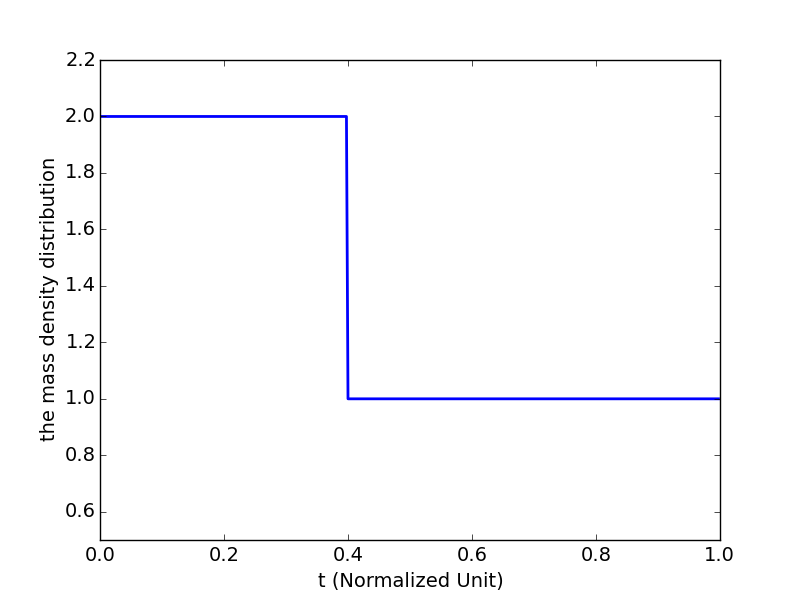
\includegraphics[width=\textwidth]{images/FexactPlot/fexactplot}
			\caption{f(t)}
			\label{fig:f(t)}
		\end{subfigure}
		\begin{subfigure}[b]{0.7\textwidth}
			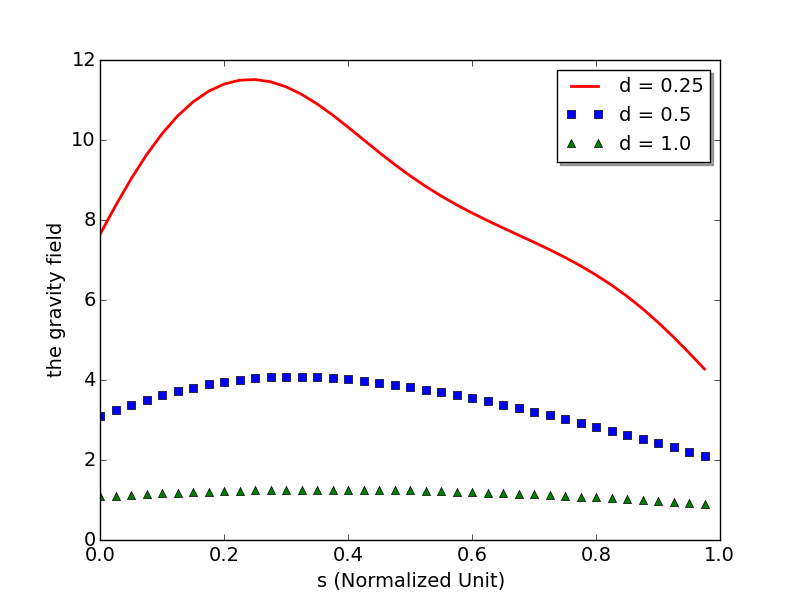
\includegraphics[width=\textwidth]{images/GexactPlot/gexactplot}
			\caption{g(s)}
			\label{fig:g(s)}
		\end{subfigure}
		\caption{(a) shows the function f(the mass density
		distribution), and (b) shows the measured signal g (the
		gravity field) for three different values of the depth d in Figure.
		\ref{fig:GeophysicsIllustrator}}\label{fig:geoexact}
\end{figure}
\subsection{Discretization of Liner Inverse Problems: Quadrature Methods}
We compute approximations \({\tilde f_j}\) to the solution f solely at selected
abscissas \({t_1},{t_2},...{t_n},i.e.\),
\[{\tilde f_j} = \tilde f({t_j}),\begin{array}{*{20}{c}}
{}&{j = 1,2,...,n.}
\end{array}\]

Quadrature methods--also called Nystrom methods--take their basis in the general
quadrature rule of the form 
\[\int\limits_0^1 {\varphi (t)dt = \sum\limits_{j = 1}^n {{\omega _j}\varphi
({t_j})} }  + {E_n}\]
where \(\varphi \) is the function whose integral we want to evaluate, \({E_n}\)
is the quadrature error, \({t_1},{t_2},...,{t_n}\) are the abscissas for the
quadrature rule, and \({\omega _1},{\omega _2},{\omega _3},...,{\omega _n}\) are
the corresponding weights. For example, for the midpoint rule in the interval
\([0, 1]\) we have
\begin{equation}
{t_j} = \frac{{j - \frac{1}{2}}}{n},\begin{array}{*{20}{c}}
{}&{{\omega _j} = \frac{1}{n},\begin{array}{*{20}{c}}
{}&{j = 1,2,...n.}
\end{array}}
\end{array}
\end{equation}
Apply the quadrature methods on Eq.\ref{eq:integralequation}, we arrive at the
relations
\begin{equation}
\sum\limits_{j = 1}^n {{\omega _j}K({s_j},{t_j})} {\tilde f_j} = g({s_i}),\begin{array}{*{20}{c}}
{}&{i = 1,...n.}
\end{array}
\end{equation}

The realtion in Eq.\ref{eq:disintegral} are just a linear system, which can be
also written as
\[\left( {\begin{array}{*{20}{c}}
{{\omega _1}K({s_1},{t_1})}&{{\omega _2}K({s_1},{t_2})}&{...}&{{\omega _n}K({s_1},{t_n})}\\
{{\omega _1}K({s_2},{t_1})}&{{\omega _2}K({s_2},{t_2})}&{...}&{{\omega _1}K({s_2},{t_n})}\\
 \vdots & \vdots &{}& \vdots \\
{{\omega _1}K({s_n},{t_1})}&{{\omega _1}K({s_n},{t_2})}&{...}&{{\omega _1}K({s_n},{t_n})}
\end{array}} \right)\]

or simply \(Ax=b\), where A is an \(n \times n\) matrix. The elements of the
matrix A, the right-hand side b, and the solution vector x are given by
\begin{equation}
\left. {\begin{array}{*{20}{c}}
{{a_{ij}} = {\omega _j}K({s_i},{t_j})}\\
{{x_j} = \tilde f({t_j})}\\
{{b_i} = g({s_i})}
\end{array}} \right\}\begin{array}{*{20}{c}}
{}&{i,j = 1,...,n.}
\end{array}
\end{equation}


\subsection{The Singular Value Decompostion}
While the matrices that we encountered in the previous section are squre, it can
be aslo apply to general case. Hence, we  assume that the matrix is either
square or has more rows than columns. Then, for any matrix \(A \in {R^{m \times
n}}\) with \(m \geqslant n\), the SVD takes the form
\begin{equation}
A = U\Sigma {V^T} = \sum\limits_{i = 1}^n {{u_i}{\sigma _i}v_i^T} 
\end{equation}
Here, \(\Sigma  \in {R^{n \times n}}\) is a diagonal matrix with the signluar
values, satisfying
\[\Sigma  = diag({\sigma _1},...,{\sigma _n}),\begin{array}{*{20}{c}}
{{\sigma _1} \ge {\sigma _2} \ge  \cdots  \ge {\sigma _n} \ge 0}&{}
\end{array}\]

The matrices \(U \in {R^{m \times n}}\) and \(V \in {R^{m \times n}}\) consistt
of the left and right singular vectors
\[U = ({u_1},...,{u_n})\begin{array}{*{20}{c}}
{}&{V = ({v_1},...,{v_n})}
\end{array}\]
and both matrices have orthonormal columns:
\[{U^T}U = {V^T}V = I\]

Here we apply the svd to the inverse problem \(x = {A^{ - 1}}b\), we immediately
see that the ``naive'' solution is given by
\begin{equation}
x = {A^{ - 1}}b = \sum\limits_{i = 1}^n {\frac{{u_i^Tb}}{{{\sigma _i}}}}
{v_i}
\end{equation}

\subsection{SVD Analysis and the Discrete Picard Condition}
The Discrete picard Condition: Let \(\tau \) denote the level at which the
computed singular values \({\sigma _i}\) level off due to rounding errors. The
discrete Picard condition is satisfied if, for all singular values larger than
\(\tau \), the correspoing coefficients \(\left| {u_i^Tb} \right|\), on average,
decay faster than the \({\sigma _i}\).

Figure.\ref{fig:picard_plot} shows the picard plot fro the discretized gravity
surveing problem with different noise level.
\begin{figure}
	\centering
		\begin{subfigure}[b]{0.7\textwidth}
			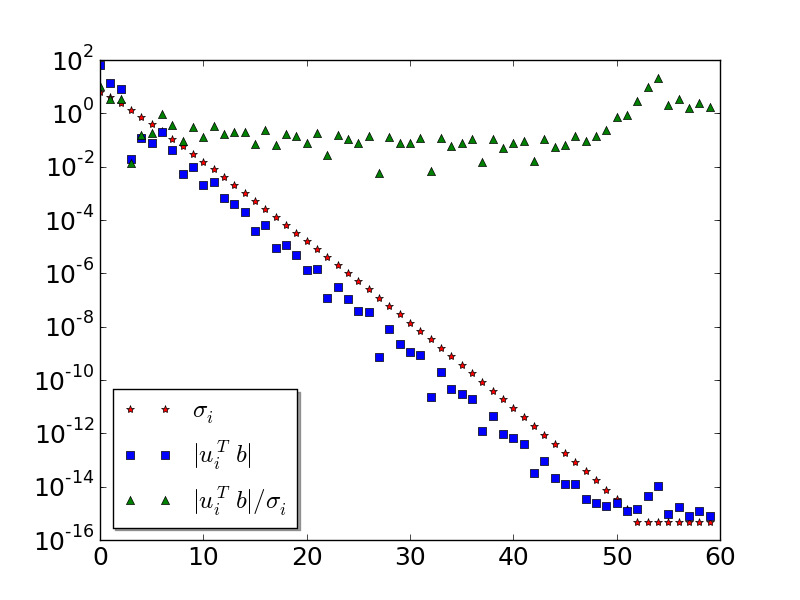
\includegraphics[width=\textwidth]{images/PicardPlot/picardplot_without_noise}
			\caption{With
			no noise in the right hand side (only discretization noise)}
		\end{subfigure}
		\begin{subfigure}[b]{0.7\textwidth}
			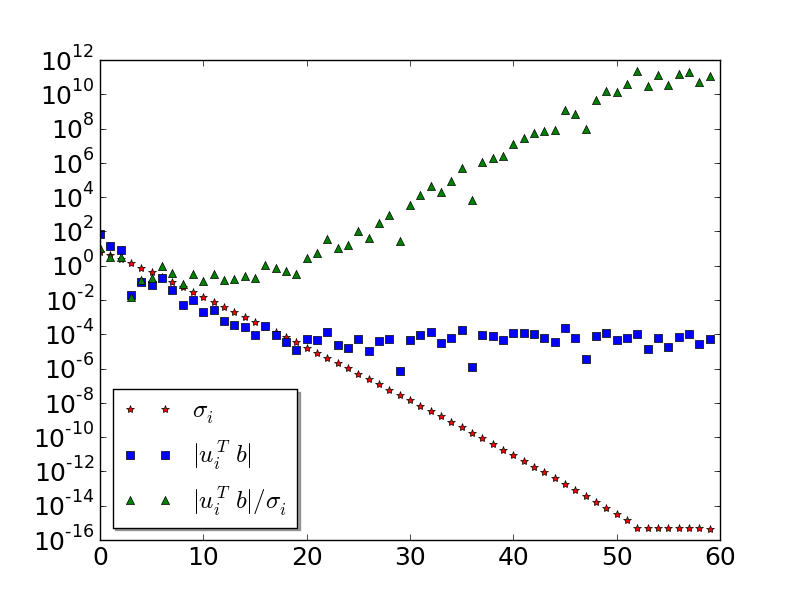
\includegraphics[width=\textwidth]{images/PicardPlot/picardplot_with_noise}
			\caption{With
			added noise in the right hand side}
		\end{subfigure}
		\caption{The Picard plots for the discretized gravity
		surveing problem with different noise level. (a) With
		no added noise (only discretization noise). (b) With
		an addional white noised added to the measured g
		(1E-4 random white noise)}\label{fig:picard_plot}
\end{figure}
\subsection{Truncated SVD}
Figure.\ref{fig:tsvd_plot} shows tsvd reconstructed f for the discretized
gravity surveing problem with differernt noise level.
\begin{figure}
	\centering
		\begin{subfigure}[b]{0.7\textwidth}
			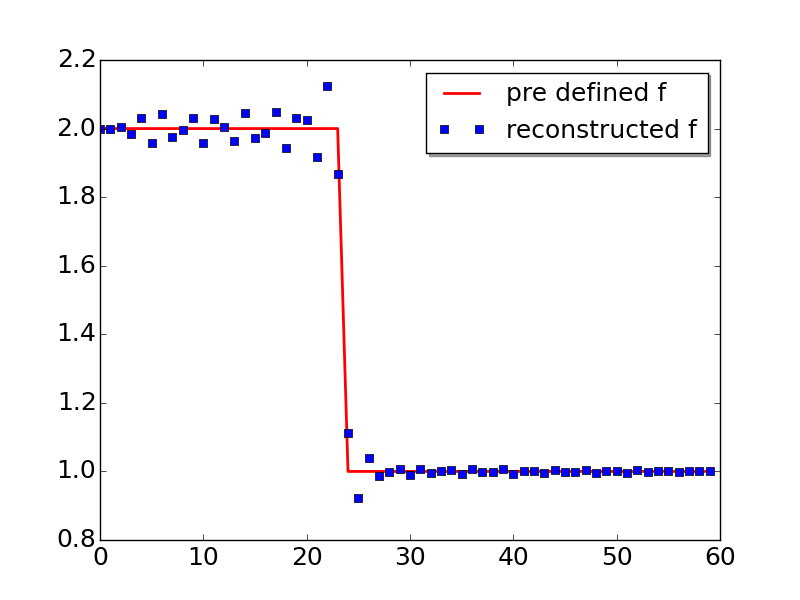
\includegraphics[width=\textwidth]{images/TSVD/tsvdplot}
			\caption{With
			no noise in the right hand side (only discretization noise) truncated number
			k = 48}
		\end{subfigure}
		\begin{subfigure}[b]{0.7\textwidth}
			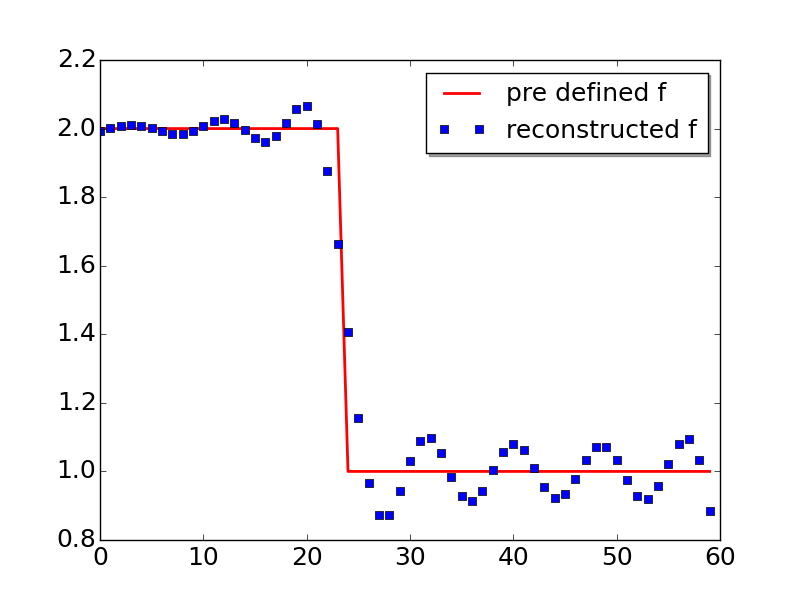
\includegraphics[width=\textwidth]{images/TSVD/tsvdplot_withnoise}
			\caption{With
			added noise in the right hand side (white noise 1E-4), truncated number k =
			18}
		\end{subfigure}
		\caption{TSVD f reconstruction}\label{fig:tsvd_plot}
\end{figure}
\subsection{Tikhonov Regularization}
Figure.\ref{fig:tikhonov_plot} shows Tikhonov Regularization reconstructed f for the
discretized gravity surveing problem with differernt noise level.
\begin{figure}
	\centering
		\begin{subfigure}[b]{0.7\textwidth}
			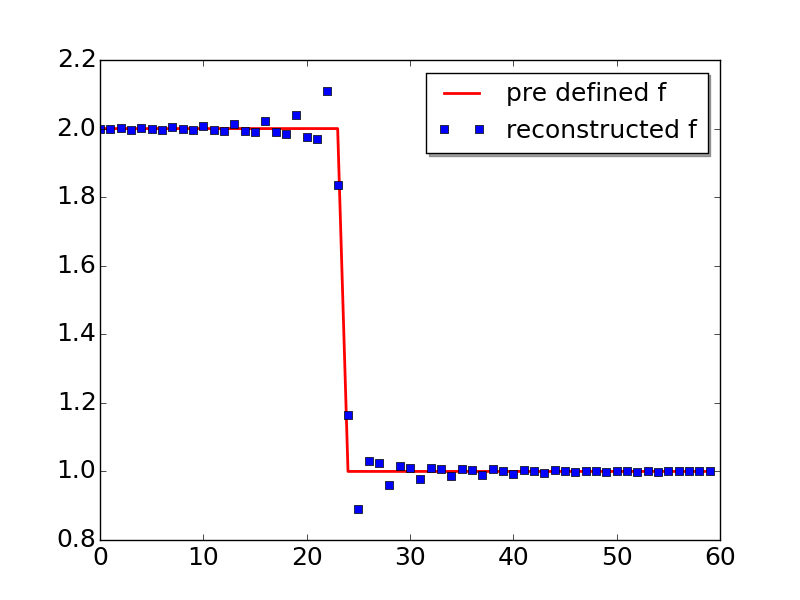
\includegraphics[width=\textwidth]{images/TikhonovRegularization/tikhonovplot}
			\caption{With
			no noise in the right hand side (only discretization noise), \(\lambda \) =
			1E-12}
		\end{subfigure}
		\begin{subfigure}[b]{0.7\textwidth}
			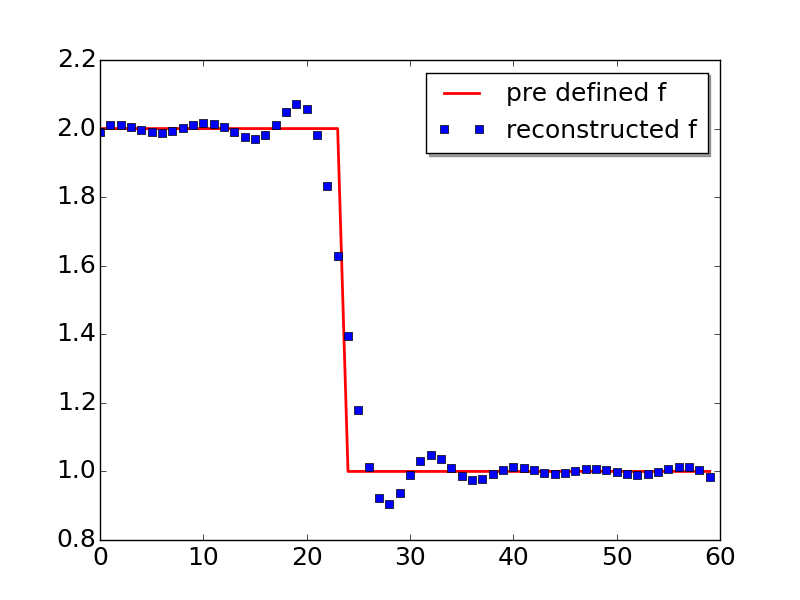
\includegraphics[width=\textwidth]{images/TikhonovRegularization/tikhonovplot_withnoise}
			\caption{With
			added noise in the right hand side (white noise 1E-4), \(\lambda \) =
			1E-3}
		\end{subfigure}
		\caption{Tikhonov Regularization f reconstruction}\label{fig:tikhonov_plot}
\end{figure}
\subsection{Fitness of the Reconstruction: Generalized Cross Validation}
The fitness is calculated as:
\begin{equation}
	\mathop {\min }\limits_\lambda  ||A{x_\lambda } - {b^{exact}}||_2^2
\end{equation}
However, we can't calculate it since \(b^{exact}\) is not available. Generalized 
Cross Validation is a classical statistical technique that comes into good use
here \cite{hansen2010discrete}.

Using Generalized Cross Validation(GSV), the fitness can be calculated as:
\begin{equation}
	\mathop {\min }\limits_\lambda  \frac{{||A{x_\lambda } - b||_2^2}}{{{{(m -
	\sum\nolimits_{i = 1}^n {\varphi _i^{[\lambda ]}} )}^2}}}
	\label{eq:disintegral}
\end{equation}
\subsection{Self Consistent Regularization With Cross Validation}

\section{Cellular Evolutionary Algorithm}
\begin{figure}
	\centering
		\begin{subfigure}[b]{0.4\textwidth}
			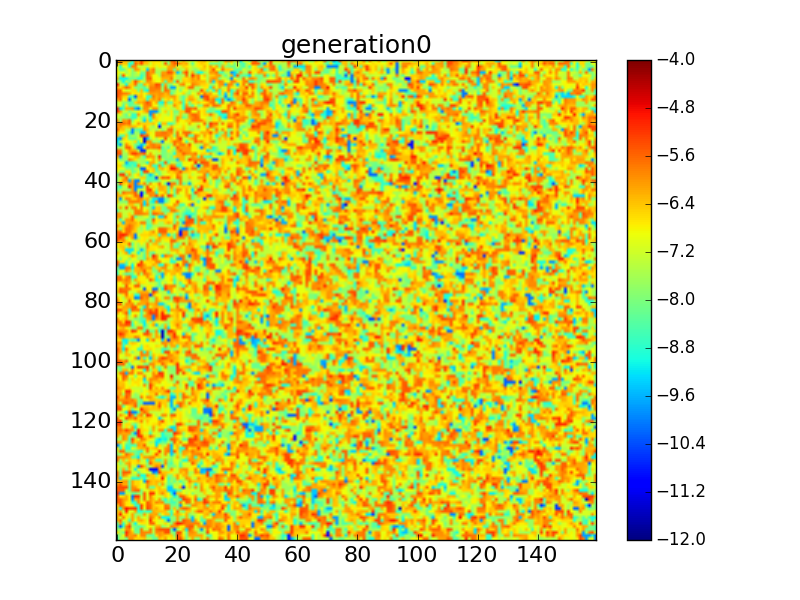
\includegraphics[width=\textwidth]{images/CEA/simulation1/generation0}
			\caption{lowest fitness = 2.60e-12}
		\end{subfigure}
		\begin{subfigure}[b]{0.4\textwidth}
			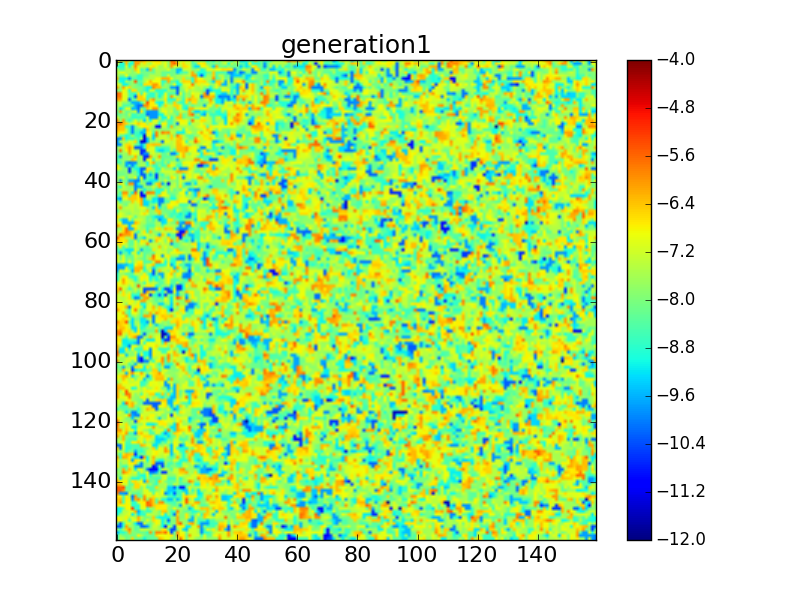
\includegraphics[width=\textwidth]{images/CEA/simulation1/generation1}
			\caption{lowest fitness = 1.65e-25}
		\end{subfigure}
		\begin{subfigure}[b]{0.4\textwidth}
			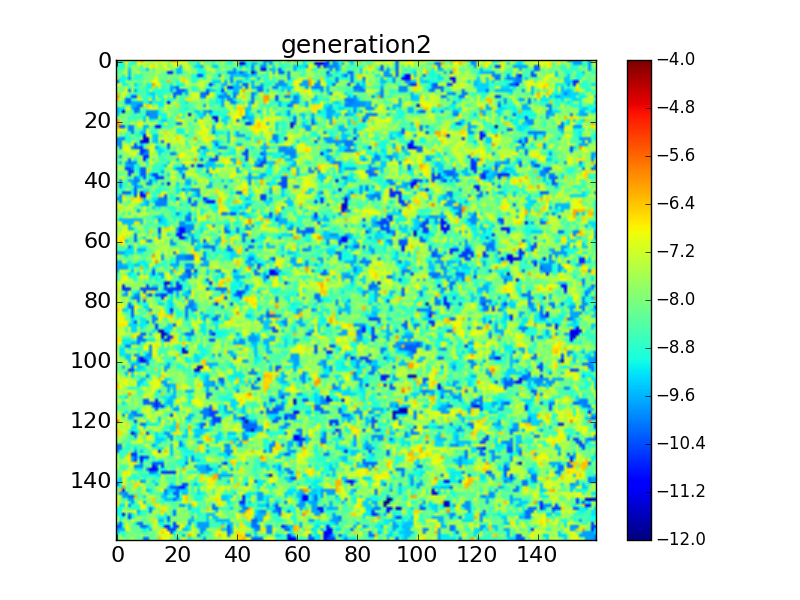
\includegraphics[width=\textwidth]{images/CEA/simulation1/generation2}
			\caption{lowest fitness = 1.65e-25}
		\end{subfigure}
		\begin{subfigure}[b]{0.4\textwidth}
			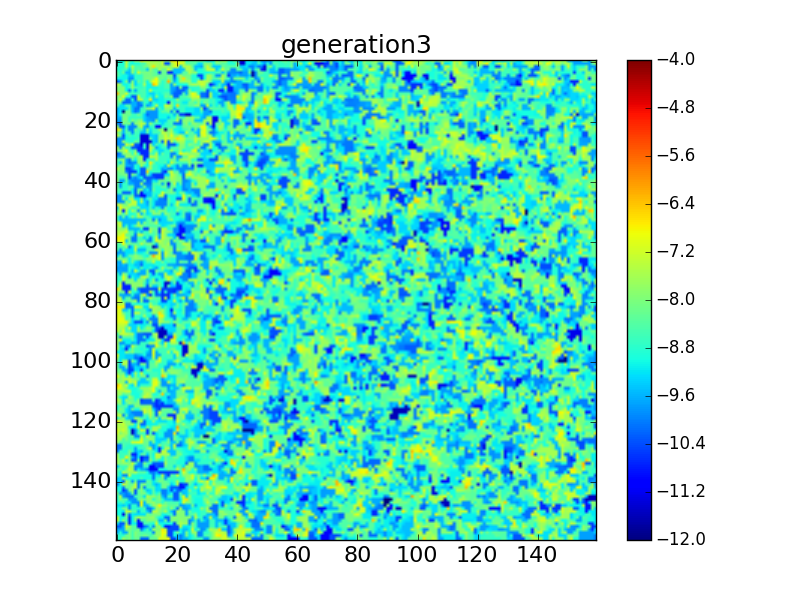
\includegraphics[width=\textwidth]{images/CEA/simulation1/generation3}
			\caption{lowest fitness = 1.65e-25}
		\end{subfigure}
		\caption{4 generation of CEA simulation fitness map, we come to the exact de
		noise measurement of only 2 generation}\label{fig:ceasimulation1}
\end{figure}
\subsection{Evolutionary Algorithms}
Evolutinary algorithms (EAs) are a family of heuristic search methods that are
often used nowadays to find satisfactory solutions to difficult optimization and
machine learning problems. EAs are lossely based on a few fundamental
evolutionary ideas introduced by Darwin in the niewteenth century. These
concepts revolve around the notion of populations of organisms adapting to their
enviroment through genetic inheritance and survivial of the fittest.

Each individual may be viewed as a representation, according to an appropriate
encoding, of a particular solution to an algorithmic problem. To implement an
EAs for solving a given problem, at least approximately, the user must provide
the following pieces of information.

\subsubsection{Representation}
Individuals in the population represent solutions to a pronlem and must be
encoded in some way to manipulated by the EA processes. They may be just string
of binary digits, which is a widespread and universal representation, or they
may be any other data structure that is suitable for the problem at hand such as
string of integers, alphabetic characters, strings of real numbers, and even
trees or graphs.
\subsubsection{Genetic Operators}

Usually Evolutionary Algorithm assume that the strucutre of the population is
panmictic, which means that any inidividual may interact with any other individual in the population.
However, this need not be always the case: we often see population sin the
biological and social world in which individuals only interact with a subset of
the rest of the population. This situation can usefully be depicated by using
the concept of a population graph \cite{hoekstra2010simulating}.

\bibliography{mybib}{}
\bibliographystyle{plain}
\end{document}
